% =====================================================================
%  SAY, ECHO, DO  --  Concept Explainer (short version)
% =====================================================================
\documentclass[11pt,a4paper]{article}

\usepackage[utf8]{inputenc}
\IfFileExists{lmodern.sty}{\usepackage[T1]{fontenc}\usepackage{lmodern}}{}
\usepackage[margin=2.5cm]{geometry}
\usepackage{amsmath,amssymb,bm}
\usepackage{booktabs,tabularx,array}
\usepackage{enumitem}
\usepackage{xcolor}
\usepackage{tikz}
\usetikzlibrary{positioning,arrows.meta,calc,decorations.markings,shapes.geometric,decorations.pathreplacing}
\usepackage{pgfplots}
\pgfplotsset{compat=1.16}
\usepgfplotslibrary{groupplots}
\usepackage[most]{tcolorbox}
\usepackage{titlesec}
\usepackage[numbers,sort&compress]{natbib}
\usepackage{microtype}
\usepackage{setspace}
\usepackage[colorlinks=true,linkcolor=blue!50!black,citecolor=blue!50!black,urlcolor=blue!50!black]{hyperref}
\usepackage[capitalise,noabbrev]{cleveref}

\setstretch{1.15}
\setlength{\parskip}{5pt}
\setlength{\parindent}{0pt}
\setlist{itemsep=3pt,topsep=4pt}

% ---------- Colours --------------------------------------------------
\definecolor{say}{HTML}{8E44AD}
\definecolor{echo}{HTML}{C0392B}
\definecolor{do}{HTML}{1F618D}
\definecolor{price}{HTML}{222222}
\definecolor{good}{HTML}{1E8449}

\titleformat{\section}{\Large\bfseries\color{do!80!black}}{\thesection}{0.8em}{}
\titleformat{\subsection}{\large\bfseries}{\thesubsection}{0.7em}{}
\titlespacing*{\section}{0pt}{16pt}{6pt}

% ---------- Boxes ----------------------------------------------------
\newtcolorbox{keyidea}[1][Key idea]{enhanced,breakable,colback=do!4,colframe=do!70!black,
  boxrule=0.6pt,arc=2pt,fonttitle=\bfseries\small,title={#1},left=8pt,right=8pt,top=5pt,bottom=5pt}
\newtcolorbox{plainwords}{enhanced,breakable,colback=good!4,colframe=good!60!black,
  boxrule=0pt,leftrule=3pt,arc=0pt,outer arc=0pt,left=8pt,top=4pt,bottom=4pt,
  fontupper=\small,before upper={\textbf{In plain words.}~}}
\newtcolorbox{mathbox}[1]{enhanced,breakable,colback=white,colframe=say!60!black,
  boxrule=0.5pt,arc=2pt,fonttitle=\bfseries\small,coltitle=white,colbacktitle=say!70!black,
  title={The math: #1},left=8pt,right=8pt,fontupper=\small}

\newcommand{\z}{\bm{z}}
\newcommand{\w}{\bm{w}}
\DeclareMathOperator{\Var}{Var}
\newcommand{\SAY}{\textcolor{say}{\textbf{Say}}}
\newcommand{\ECHO}{\textcolor{echo}{\textbf{Echo}}}
\newcommand{\DO}{\textcolor{do}{\textbf{Do}}}

% =====================================================================
\begin{document}

\begin{center}
{\Huge\bfseries \textcolor{say}{Say}, \textcolor{echo}{Echo}, \textcolor{do}{Do}\par}
\vspace{4pt}
{\large Reading the gap between what markets hear and what money does\par}
\vspace{6pt}
{\normalsize A concept explainer \quad$\cdot$\quad [Author Name] \quad$\cdot$\quad September 2026\par}
\end{center}

\vspace{4pt}
\begin{tcolorbox}[enhanced,colback=gray!4,colframe=gray!40,boxrule=0.4pt,arc=2pt,left=10pt,right=10pt]
\small
\textbf{Summary.} Markets hear three voices. Institutions \emph{say} things. The media \emph{echoes} them. Capital \emph{does} things. Most sentiment models listen only to the first two. This explainer describes a framework that listens for \emph{disagreement} between the voices, using AI embeddings to read what the narrative really means and quantitative finance to read what money is really doing. It rests on two inversions: \emph{trust deeds over words}, and \emph{fade the echo, follow the news}.
\end{tcolorbox}

% =====================================================================
\section{The Idea}

Everyone in markets has seen this pattern. A respected bank publishes a gloomy call. Headlines multiply. The stock drops, but less than the noise suggests, and weeks later it is higher than before. Looking back, someone was buying all along.

It is tempting to call this a conspiracy. We don't need to. We only need to \emph{measure the disagreement} between three voices:

\begin{center}
\small
\begin{tabular}{@{}>{\raggedright}p{1.6cm}>{\raggedright}p{4.8cm}>{\raggedright\arraybackslash}p{6.8cm}@{}}
\toprule
Voice & What it is & Where we see it \\
\midrule
\SAY & What institutions publicly claim & Ratings, target changes, research notes, management tone, interviews \\
\ECHO & What the media repeats & News volume, syndication, social posts, emotional intensity \\
\DO & What capital actually does & Holdings, futures positioning, insider trades, options flow, price \\
\bottomrule
\end{tabular}
\end{center}

\begin{figure}[ht]
\centering
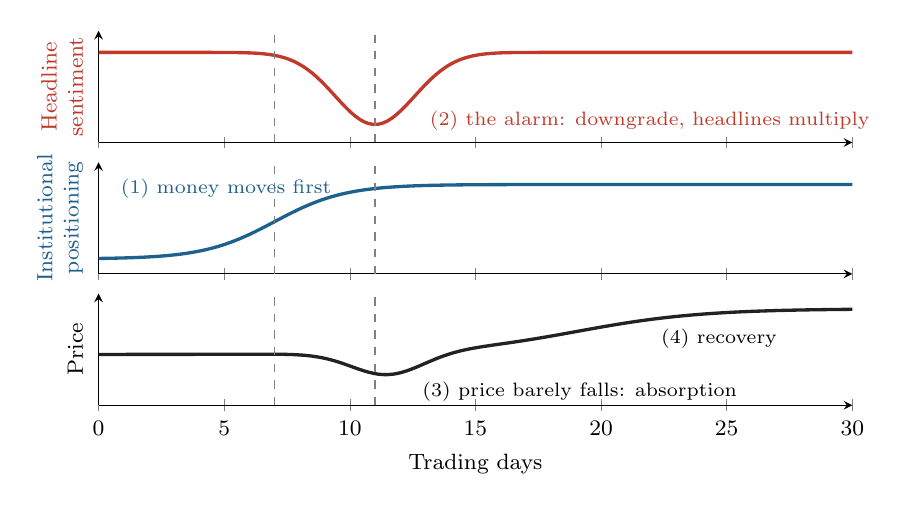
\begin{tikzpicture}
\begin{groupplot}[
  group style={group size=1 by 3, vertical sep=0.25cm, xticklabels at=edge bottom},
  width=0.92\textwidth, height=3.0cm,
  xmin=0, xmax=30, axis lines=left, ytick=\empty,
  xtick={0,5,...,30}, no markers, samples=160, domain=0:30,
  ylabel style={align=center, font=\footnotesize},
  tick label style={font=\footnotesize}, clip=false]
\nextgroupplot[ylabel={\textcolor{echo}{Headline}\\\textcolor{echo}{sentiment}}, ymin=-1.25, ymax=0.3]
  \addplot[echo, very thick] {-exp(-((x-11)^2)/5)};
  \addplot[gray, dashed] coordinates {(7,-1.25) (7,0.3)};
  \addplot[gray, dashed] coordinates {(11,-1.25) (11,0.3)};
  \node[font=\scriptsize, anchor=west, text=echo] at (axis cs:12.8,-0.95) {(2) the alarm: downgrade, headlines multiply};
\nextgroupplot[ylabel={\textcolor{do}{Institutional}\\\textcolor{do}{positioning}}, ymin=-0.2, ymax=1.3]
  \addplot[do, very thick] {1/(1+exp(-(x-7)/1.4))};
  \addplot[gray, dashed] coordinates {(7,-0.2) (7,1.3)};
  \addplot[gray, dashed] coordinates {(11,-0.2) (11,1.3)};
  \node[font=\scriptsize, anchor=west, text=do] at (axis cs:0.5,0.95) {(1) money moves first};
\nextgroupplot[ylabel={Price}, ymin=95, ymax=106, xlabel={\footnotesize Trading days}]
  \addplot[price, very thick] {100 - 2.2*exp(-((x-11.5)^2)/4) + 4.5/(1+exp(-(x-19)/2.5))};
  \addplot[gray, dashed] coordinates {(7,95) (7,106)};
  \addplot[gray, dashed] coordinates {(11,95) (11,106)};
  \node[font=\scriptsize, anchor=west] at (axis cs:12.5,96.3) {(3) price barely falls: absorption};
  \node[font=\scriptsize, anchor=west] at (axis cs:22,101.6) {(4) recovery};
\end{groupplot}
\end{tikzpicture}
\caption{The false-alarm pattern (stylised). Positioning builds (1) before the alarm (2); the price falls far less than the alarm implies (3), then recovers (4).}
\label{fig:pattern}
\end{figure}

\begin{keyidea}[The two inversions]
\textbf{1. Deeds over words.} When \SAY\ and \DO\ disagree, trust \DO. A bearish institutional call accompanied by institutional buying is a bullish signal.

\textbf{2. Fade the echo, follow the news.} Split media sentiment into \emph{new information} and \emph{echo}. Prices tend to drift after real news; it is the amplification that overshoots.
\end{keyidea}

The price is the referee. If the story says the stock should fall 6\% and it falls 2\%, someone absorbed the selling. And the logic runs both ways: euphoric coverage while institutions quietly sell is the mirror image at market tops. The framework never assumes ``always be contrarian''; it asks which of four situations we are in.

\begin{figure}[ht]
\centering
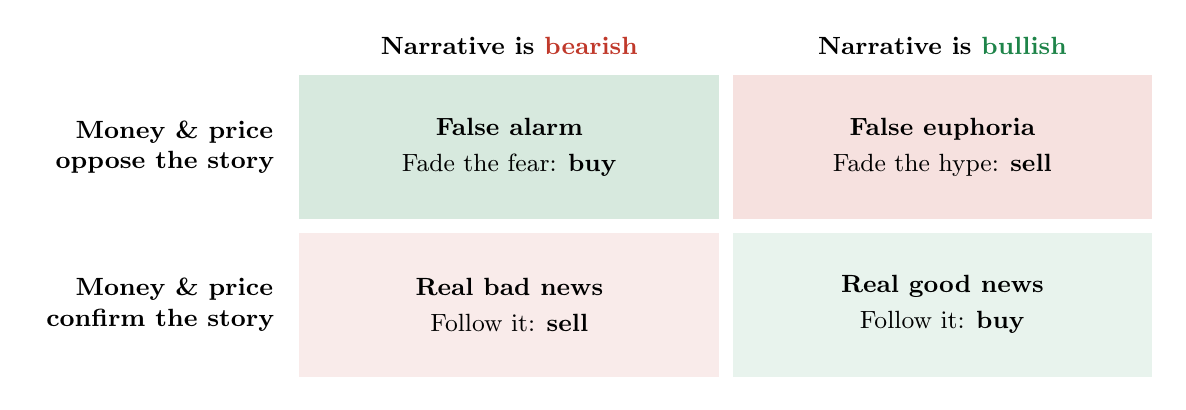
\begin{tikzpicture}[
  cell/.style={draw=white, line width=2pt, minimum width=5.4cm, minimum height=1.9cm, align=center, font=\small},
  head/.style={font=\small\bfseries, align=center}]
\node[cell, fill=good!18] (a) at (0,0) {\textbf{False alarm}\\[2pt] Fade the fear: \textbf{buy}};
\node[cell, fill=echo!15] (b) at (5.5,0) {\textbf{False euphoria}\\[2pt] Fade the hype: \textbf{sell}};
\node[cell, fill=echo!10] (c) at (0,-2.0) {\textbf{Real bad news}\\[2pt] Follow it: \textbf{sell}};
\node[cell, fill=good!10] (d) at (5.5,-2.0) {\textbf{Real good news}\\[2pt] Follow it: \textbf{buy}};
\node[head, above=2pt of a] {Narrative is \textcolor{echo}{bearish}};
\node[head, above=2pt of b] {Narrative is \textcolor{good}{bullish}};
\node[head, left=4pt of a, text width=3.0cm, align=right] {Money \& price\\ \textbf{oppose} the story};
\node[head, left=4pt of c, text width=3.0cm, align=right] {Money \& price\\ \textbf{confirm} the story};
\end{tikzpicture}
\caption{The decision matrix. The narrative alone never decides the trade; its agreement with money and price does.}
\label{fig:matrix}
\end{figure}

% =====================================================================
\section{Why Inverting Sentiment Can Work}

The ingredients are well established. Media pessimism creates short-term pressure that later reverses \citep{tetlock2007}. Attention-grabbing news pulls in less-informed buyers \citep{barber2008}. Sentiment can push prices away from value because betting against it is risky \citep{delong1990,shleifer1997}. Sophisticated traders profit by trading against forced or emotional flow \citep{brunnermeier2005}. Yet prices also \emph{drift} after genuine news \citep{chan2003}, which is why a naive contrarian rule fails.

A tiny model makes the logic precise. A stock is worth $v$; a narrative $m = v + \text{noise}$ arrives; the crowd moves the price by $\varphi$ per unit of narrative, while a rational observer would use weight $w^\star = \Var(v)/\Var(m)$.

\begin{figure}[ht]
\centering
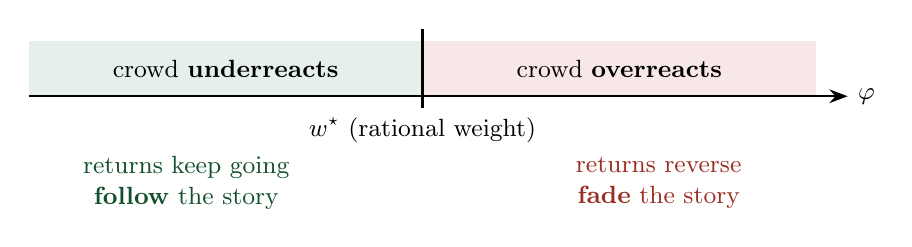
\begin{tikzpicture}[font=\small]
\fill[good!12] (0,0) rectangle (5,0.7);
\fill[echo!12] (5,0) rectangle (10,0.7);
\draw[thick,-{Stealth}] (0,0) -- (10.4,0) node[right] {$\varphi$};
\draw[very thick] (5,-0.15) -- (5,0.85);
\node[below] at (5,-0.15) {$w^\star$ (rational weight)};
\node[align=center] at (2.5,0.35) {crowd \textbf{underreacts}};
\node[align=center] at (7.5,0.35) {crowd \textbf{overreacts}};
\node[align=center, text=good!60!black] at (2.0,-1.1) {returns keep going\\ \textbf{follow} the story};
\node[align=center, text=echo!80!black] at (8.0,-1.1) {returns reverse\\ \textbf{fade} the story};
\end{tikzpicture}
\caption{Result 1. Whether to follow or fade the narrative depends on one comparison: how strongly the crowd reacts versus how much the narrative is actually worth.}
\label{fig:phi}
\end{figure}

The model gives three results:
\begin{enumerate}[label=\textbf{Result \arabic*.},leftmargin=*]
  \item Fade the story \emph{only} when the crowd overreacts (\cref{fig:phi}).
  \item The price move \emph{net of} what the narrative implied reveals the hidden informed trader, and it predicts continuation in its own direction.
  \item Any observation of real positioning, however noisy, makes the forecast sharper.
\end{enumerate}

% =====================================================================
\section{Embeddings: A Map of Meaning}

An embedding model turns text into a point in a high-dimensional space, so that texts with similar meaning land close together. Think of it as a \emph{map of meaning}. On this map, \textbf{directions carry concepts} (moving one way makes text more alarming) and \textbf{distances carry surprise} (how far the story landed from where it was expected to land).

\begin{figure}[ht]
\centering
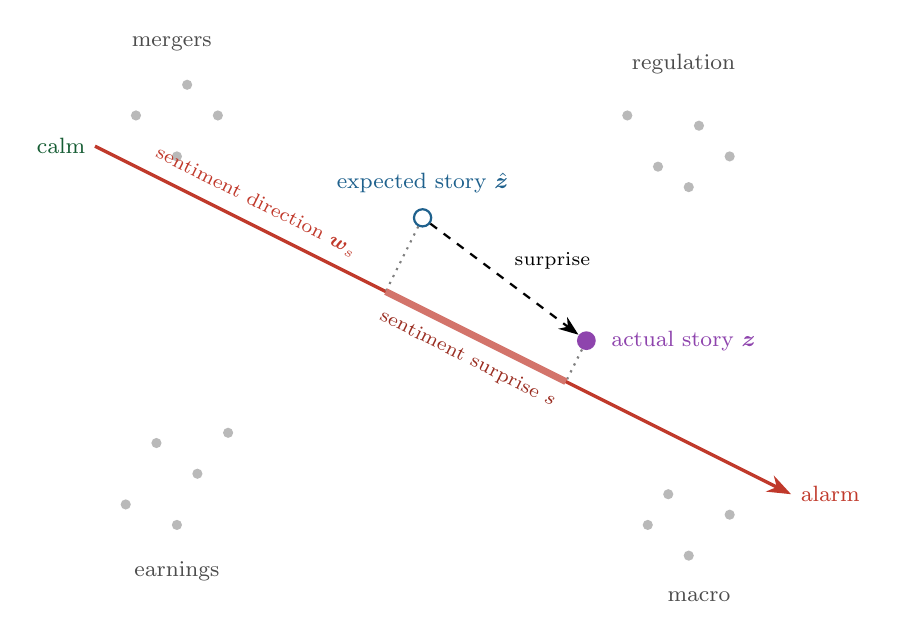
\begin{tikzpicture}[scale=1.3, dot/.style={circle, fill=gray!55, inner sep=1.3pt}]
\foreach \p in {(-2.6,-1.3),(-2.2,-1.6),(-2.9,-1.9),(-2.4,-2.1),(-1.9,-1.2)} \node[dot] at \p {};
\node[font=\footnotesize, text=gray!60!black] at (-2.4,-2.55) {earnings};
\foreach \p in {(-2.4,1.5),(-2.0,1.9),(-2.8,1.9),(-2.3,2.2)} \node[dot] at \p {};
\node[font=\footnotesize, text=gray!60!black] at (-2.45,2.6) {mergers};
\foreach \p in {(2.3,1.4),(2.7,1.8),(2.0,1.9),(2.6,1.2),(3.0,1.5)} \node[dot] at \p {};
\node[font=\footnotesize, text=gray!60!black] at (2.55,2.4) {regulation};
\foreach \p in {(2.2,-2.1),(2.6,-2.4),(3.0,-2.0),(2.4,-1.8)} \node[dot] at \p {};
\node[font=\footnotesize, text=gray!60!black] at (2.7,-2.8) {macro};
\draw[-{Stealth[length=3mm]}, echo, very thick] (-3.2,1.6) -- (3.6,-1.8);
\node[font=\footnotesize, text=echo, anchor=west] at (3.6,-1.8) {alarm};
\node[font=\footnotesize, text=good!70!black, anchor=east] at (-3.2,1.6) {calm};
\node[font=\scriptsize, text=echo, rotate=-26.6, anchor=south] at (-1.7,0.9) {sentiment direction $\w_s$};
\node[circle, draw=do, thick, fill=white, inner sep=2.2pt] (ez) at (0,0.9) {};
\node[circle, fill=say, inner sep=2.4pt] (az) at (1.6,-0.3) {};
\node[font=\footnotesize, text=do, anchor=south] at (0,1.05) {expected story $\hat{\z}$};
\node[font=\footnotesize, text=say, anchor=west] at (1.75,-0.3) {actual story $\z$};
\draw[-{Stealth[length=2.5mm]}, dashed, thick] (ez) -- (az) node[midway, above right, font=\scriptsize] {surprise};
\draw[dotted, thick, gray] (ez) -- (-0.36,0.18);
\draw[dotted, thick, gray] (az) -- (1.40,-0.70);
\draw[line width=2.5pt, echo!70] (-0.36,0.18) -- (1.40,-0.70);
\node[font=\scriptsize, text=echo!80!black, rotate=-26.6, anchor=north] at (0.52,-0.32) {sentiment surprise $s$};
\end{tikzpicture}
\caption{The map of meaning (a 2D cartoon of a 1024-dimensional space). Stories cluster by topic. Sentiment is a direction from calm to alarm. Surprise is the gap between the expected and the actual story, and \emph{sentiment surprise} is the part of that gap along the alarm direction.}
\label{fig:map}
\end{figure}

\subsection{Teaching the map what matters to markets}

Off-the-shelf embeddings organise text by \emph{topic}: two oil stories sit together whether they turned out bullish or bearish. We fine-tune the model on history so that stories with similar \emph{market aftermaths} move together (\cref{fig:finetune}). After training, ``this kind of news tends to be overdone'' becomes a place on the map.

\begin{figure}[ht]
\centering
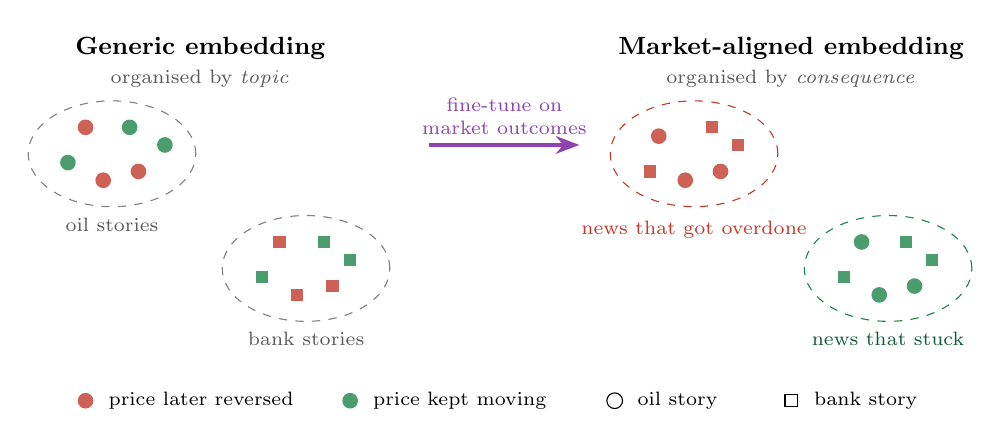
\begin{tikzpicture}[scale=1.12,
  cr/.style={circle, fill=echo!80, inner sep=2pt},
  cg/.style={circle, fill=good!80, inner sep=2pt},
  sr/.style={rectangle, fill=echo!80, inner sep=2.2pt},
  sg/.style={rectangle, fill=good!80, inner sep=2.2pt}]
% left panel
\node[font=\small\bfseries] at (2.3,3.4) {Generic embedding};
\node[font=\scriptsize, text=gray!70!black] at (2.3,3.05) {organised by \emph{topic}};
\draw[dashed, gray] (1.3,2.2) ellipse (0.95 and 0.6);
\draw[dashed, gray] (3.5,0.9) ellipse (0.95 and 0.6);
\node[font=\scriptsize, text=gray!70!black] at (1.3,1.4) {oil stories};
\node[font=\scriptsize, text=gray!70!black] at (3.5,0.1) {bank stories};
\foreach \p in {(1.0,2.5),(1.6,2.0),(1.2,1.9)} \node[cr] at \p {};
\foreach \p in {(1.5,2.5),(0.8,2.1),(1.9,2.3)} \node[cg] at \p {};
\foreach \p in {(3.2,1.2),(3.8,0.7),(3.4,0.6)} \node[sr] at \p {};
\foreach \p in {(3.7,1.2),(3.0,0.8),(4.0,1.0)} \node[sg] at \p {};
% arrow
\draw[-{Stealth[length=3mm]}, very thick, say] (4.9,2.3) -- (6.6,2.3) node[midway, above, font=\scriptsize, align=center] {fine-tune on\\ market outcomes};
% right panel
\node[font=\small\bfseries] at (9.0,3.4) {Market-aligned embedding};
\node[font=\scriptsize, text=gray!70!black] at (9.0,3.05) {organised by \emph{consequence}};
\draw[dashed, echo] (7.9,2.2) ellipse (0.95 and 0.6);
\draw[dashed, good] (10.1,0.9) ellipse (0.95 and 0.6);
\node[font=\scriptsize, text=echo, anchor=north] at (7.9,1.55) {news that got overdone};
\node[font=\scriptsize, text=good!70!black] at (10.1,0.1) {news that stuck};
\foreach \p in {(7.5,2.4),(8.2,2.0),(7.8,1.9)} \node[cr] at \p {};
\foreach \p in {(8.1,2.5),(7.4,2.0),(8.4,2.3)} \node[sr] at \p {};
\foreach \p in {(9.8,1.2),(10.4,0.7),(10.0,0.6)} \node[cg] at \p {};
\foreach \p in {(10.3,1.2),(9.6,0.8),(10.6,1.0)} \node[sg] at \p {};
% legend
\node[cr] at (1.0,-0.6) {}; \node[font=\scriptsize, anchor=west] at (1.15,-0.6) {price later reversed};
\node[cg] at (4.0,-0.6) {}; \node[font=\scriptsize, anchor=west] at (4.15,-0.6) {price kept moving};
\node[circle, draw, inner sep=2pt] at (7.0,-0.6) {}; \node[font=\scriptsize, anchor=west] at (7.15,-0.6) {oil story};
\node[rectangle, draw, inner sep=2.2pt] at (9.0,-0.6) {}; \node[font=\scriptsize, anchor=west] at (9.15,-0.6) {bank story};
\end{tikzpicture}
\caption{What fine-tuning does. Before, stories cluster by subject and good and bad outcomes are mixed. After, stories cluster by what happened next, across subjects.}
\label{fig:finetune}
\end{figure}

\begin{mathbox}{scoring a story}
Each document becomes an embedding $\z$. A small sequence model predicts the \emph{expected} next story $\hat\z$ from recent coverage and market conditions. Then
\[
\underbrace{\bm\varepsilon = \z - \hat\z}_{\text{surprise}},\qquad
\underbrace{s = \langle \w_s, \bm\varepsilon\rangle}_{\text{sentiment surprise}},\qquad
\w_s \text{ with topic directions removed.}
\]
Fine-tuning uses a contrastive loss that pulls together stories whose subsequent returns, volume and volatility were similar \citep{oord2018}.
\end{mathbox}

\begin{plainwords}
We score news on how much worse or better it is than what the market was bracing for, not on how negative it sounds.
\end{plainwords}

% =====================================================================
\section{Inversion 1: Fade the Echo, Follow the News}

When one story appears and forty copies follow, the copies add attention but no information. We model story arrivals as a \emph{self-exciting} process: each story briefly raises the chance of more stories \citep{hawkes1971,bacry2015}. The model then tells us, for every story, the probability that it was \emph{new} rather than \emph{triggered} by earlier coverage.

\begin{figure}[ht]
\centering
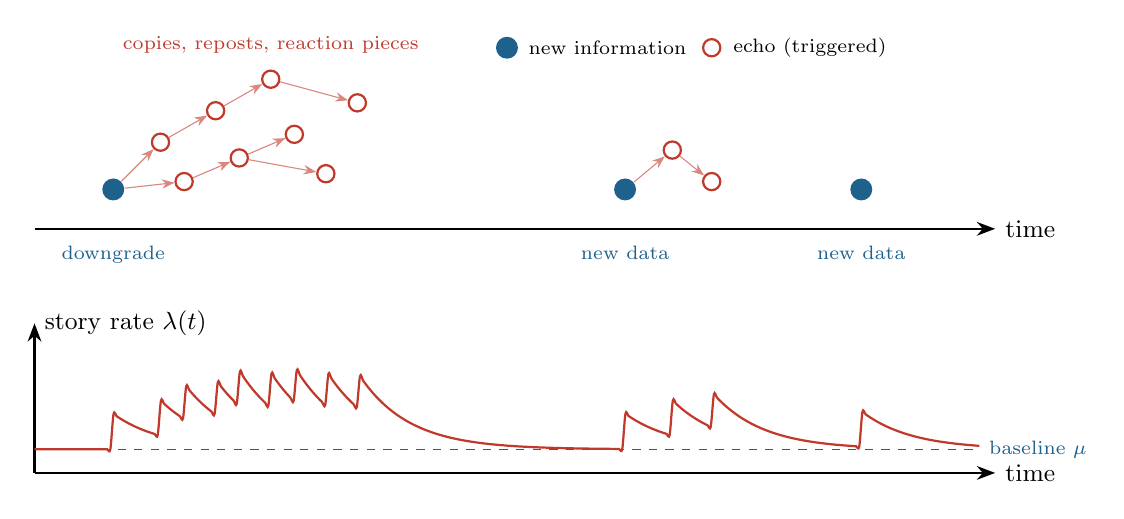
\begin{tikzpicture}[
  newn/.style={circle, fill=do, inner sep=2.8pt},
  echn/.style={circle, draw=echo, thick, fill=white, inner sep=2.2pt},
  trig/.style={-{Stealth[length=1.6mm]}, echo!60, thin}]
% time axis for cascade
\draw[-{Stealth}, thick] (0,0) -- (12.2,0) node[right, font=\small] {time};
% first cascade
\node[newn] (a) at (1,0.5) {};
\node[echn] (a1) at (1.6,1.1) {};
\node[echn] (a2) at (1.9,0.6) {};
\node[echn] (a3) at (2.3,1.5) {};
\node[echn] (a4) at (2.6,0.9) {};
\node[echn] (a5) at (3.0,1.9) {};
\node[echn] (a6) at (3.3,1.2) {};
\node[echn] (a7) at (3.7,0.7) {};
\node[echn] (a8) at (4.1,1.6) {};
\draw[trig] (a) -- (a1); \draw[trig] (a) -- (a2); \draw[trig] (a1) -- (a3);
\draw[trig] (a2) -- (a4); \draw[trig] (a3) -- (a5); \draw[trig] (a4) -- (a6);
\draw[trig] (a4) -- (a7); \draw[trig] (a5) -- (a8);
% second cascade
\node[newn] (b) at (7.5,0.5) {};
\node[echn] (b1) at (8.1,1.0) {};
\node[echn] (b2) at (8.6,0.6) {};
\draw[trig] (b) -- (b1); \draw[trig] (b1) -- (b2);
% lone new story
\node[newn] (c) at (10.5,0.5) {};
% labels
\node[font=\scriptsize, text=do, anchor=north] at (1,-0.1) {downgrade};
\node[font=\scriptsize, text=echo, anchor=south] at (3.0,2.1) {copies, reposts, reaction pieces};
\node[font=\scriptsize, text=do, anchor=north] at (7.5,-0.1) {new data};
\node[font=\scriptsize, text=do, anchor=north] at (10.5,-0.1) {new data};
% intensity curve
\begin{scope}[yshift=-3.1cm]
\draw[-{Stealth}, thick] (0,0) -- (12.2,0) node[right, font=\small] {time};
\draw[-{Stealth}, thick] (0,0) -- (0,1.9) node[right, font=\small] {story rate $\lambda(t)$};
\draw[dashed, do] (0,0.3) -- (12,0.3) node[right, font=\scriptsize, text=do] {baseline $\mu$};
\draw[echo, thick, smooth, samples=300, domain=0:12] plot (\x, {0.3
  + 0.45*(\x>1.0)*exp(-1.6*max(\x-1.0,0)) + 0.45*(\x>1.6)*exp(-1.6*max(\x-1.6,0))
  + 0.45*(\x>1.9)*exp(-1.6*max(\x-1.9,0)) + 0.45*(\x>2.3)*exp(-1.6*max(\x-2.3,0))
  + 0.45*(\x>2.6)*exp(-1.6*max(\x-2.6,0)) + 0.45*(\x>3.0)*exp(-1.6*max(\x-3.0,0))
  + 0.45*(\x>3.3)*exp(-1.6*max(\x-3.3,0)) + 0.45*(\x>3.7)*exp(-1.6*max(\x-3.7,0))
  + 0.45*(\x>4.1)*exp(-1.6*max(\x-4.1,0)) + 0.45*(\x>7.5)*exp(-1.6*max(\x-7.5,0))
  + 0.45*(\x>8.1)*exp(-1.6*max(\x-8.1,0)) + 0.45*(\x>8.6)*exp(-1.6*max(\x-8.6,0))
  + 0.45*(\x>10.5)*exp(-1.6*max(\x-10.5,0))});
\end{scope}
% legend
\node[newn] at (6.0,2.3) {}; \node[font=\scriptsize, anchor=west] at (6.15,2.3) {new information};
\node[echn] at (8.6,2.3) {}; \node[font=\scriptsize, anchor=west] at (8.75,2.3) {echo (triggered)};
\end{tikzpicture}
\caption{Echo versus news. Top: each new story (blue) can trigger a cascade of echoes (red). Bottom: the story rate jumps with every arrival and decays back to the baseline. The first episode is mostly echo; the later ones are mostly news.}
\label{fig:cascade}
\end{figure}

\begin{mathbox}{splitting sentiment}
Story arrivals follow $\lambda(t) = \mu + \sum_{\tau_j<t}\alpha\, e^{-\beta(t-\tau_j)}$. The probability that story $j$ was new is $p_j = \mu/\lambda(\tau_j)$, which splits total sentiment into
\[
s^{\text{new}} = \sum_j p_j\, s_j \quad\text{(follow)}, \qquad
s^{\text{echo}} = \sum_j (1-p_j)\, s_j \quad\text{(fade)}.
\]
The ratio $\alpha/\beta$ is the share of coverage that is echo; near 1, the narrative is feeding on itself.
\end{mathbox}

% =====================================================================
\section{Inversion 2: Deeds over Words}

The most useful comparisons match the \emph{same kind of actor} on both sides:

\begin{center}
\small
\begin{tabularx}{\textwidth}{@{}lXX@{}}
\toprule
Actor & \SAY & \DO \\
\midrule
Management & Tone on the earnings call & Insider purchases and sales \\
Asset managers & Public outlooks and interviews & Quarterly holdings disclosures \\
Futures participants & Published macro views & Weekly positioning reports \\
The market & Analyst ratings and targets & Options flow, skew, fund flows, short interest \\
\bottomrule
\end{tabularx}
\end{center}

Plot every event by what was said against what was done (\cref{fig:saydo}). Events near the diagonal are consistent: follow them. Events far off the diagonal are where the signal lives.

\begin{figure}[ht]
\centering
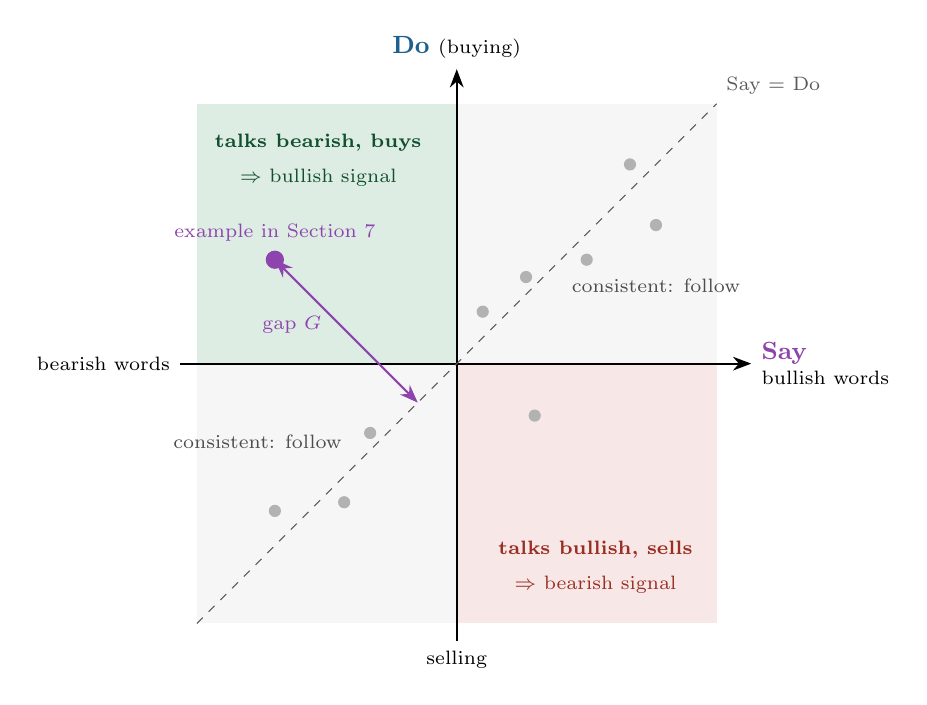
\begin{tikzpicture}[scale=1.1]
\fill[good!15] (-3,0) rectangle (0,3);
\fill[echo!12] (0,-3) rectangle (3,0);
\fill[gray!7] (0,0) rectangle (3,3);
\fill[gray!7] (-3,-3) rectangle (0,0);
\draw[-{Stealth}, thick] (-3.2,0) -- (3.4,0) node[right, font=\small, align=left] {\SAY\\[-2pt]\scriptsize bullish words};
\draw[-{Stealth}, thick] (0,-3.2) -- (0,3.4) node[above, font=\small, align=center] {\DO\ \scriptsize (buying)};
\node[font=\scriptsize, anchor=east] at (-3.2,0) {bearish words};
\node[font=\scriptsize, anchor=north] at (0,-3.2) {selling};
\draw[dashed, gray!70!black] (-3,-3) -- (3,3) node[above right, font=\scriptsize, text=gray!70!black] {Say = Do};
\node[font=\scriptsize\bfseries, text=good!60!black, align=center] at (-1.6,2.55) {talks bearish, buys};
\node[font=\scriptsize, text=good!60!black, align=center] at (-1.6,2.15) {$\Rightarrow$ bullish signal};
\node[font=\scriptsize\bfseries, text=echo!80!black, align=center] at (1.6,-2.15) {talks bullish, sells};
\node[font=\scriptsize, text=echo!80!black, align=center] at (1.6,-2.55) {$\Rightarrow$ bearish signal};
\node[font=\scriptsize, text=gray!60!black, align=center] at (2.3,0.9) {consistent: follow};
\node[font=\scriptsize, text=gray!60!black, align=center] at (-2.3,-0.9) {consistent: follow};
\foreach \p in {(0.8,1.0),(1.5,1.2),(2.0,2.3),(-1.0,-0.8),(-2.1,-1.7),(0.3,0.6),(-1.3,-1.6),(2.3,1.6),(0.9,-0.6)}
  \fill[gray!60] \p circle (2pt);
\fill[say] (-2.1,1.2) circle (3pt);
\node[font=\scriptsize, text=say, anchor=south] at (-2.1,1.3) {example in Section 7};
\draw[{Stealth}-{Stealth}, say, thick] (-2.1,1.2) -- (-0.45,-0.45);
\node[font=\scriptsize, text=say, anchor=east] at (-1.45,0.45) {gap $G$};
\end{tikzpicture}
\caption{The Say--Do plane. The distance from the diagonal is the Say--Do gap. Top-left is the false-alarm zone; bottom-right is the false-euphoria zone.}
\label{fig:saydo}
\end{figure}

Two technical pieces make this work:
\begin{itemize}
  \item \textbf{Recovering hidden positioning.} Disclosures arrive at different speeds: insider trades within days, futures positions weekly, fund holdings quarterly and weeks late. A \emph{Kalman filter} treats true positioning as a hidden quantity and each disclosure as a delayed, noisy snapshot of it. It outputs the best current estimate \emph{and} how uncertain it is, so stale data is automatically trusted less.
  \item \textbf{A credibility ledger.} Every source keeps a running track record. Reliable voices get more weight; reliably \emph{wrong} voices are not ignored, their sign is flipped. The inversion is earned from data, not assumed.
\end{itemize}

% =====================================================================
\section{Reading the Price}

\subsection{Absorption: how much the price refused to move}

The map of meaning lets us ask: \emph{when similar stories hit in similar conditions, how did prices react?} Averaging the reactions of the nearest historical analogues gives the \emph{expected} reaction. Absorption is the gap between expected and actual (\cref{fig:absorb}).

\begin{figure}[ht]
\centering
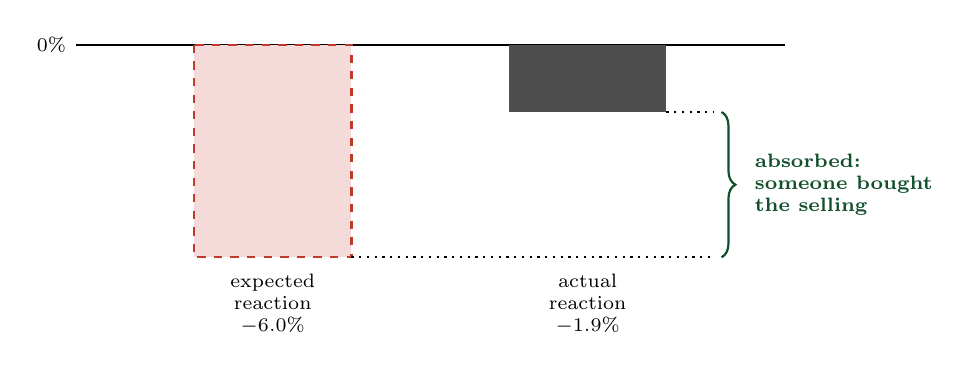
\begin{tikzpicture}[yscale=0.45, font=\small]
\draw[thick] (-0.5,0) -- (8.5,0);
\node[anchor=east, font=\scriptsize] at (-0.5,0) {0\%};
\fill[echo!18] (1,0) rectangle (3,-6);
\draw[echo, thick, dashed] (1,0) rectangle (3,-6);
\node[font=\scriptsize, align=center, anchor=north] at (2,-6.2) {expected\\ reaction\\ $-6.0\%$};
\fill[price!80] (5,0) rectangle (7,-1.9);
\node[font=\scriptsize, align=center, anchor=north] at (6,-6.2) {actual\\ reaction\\ $-1.9\%$};
\draw[dotted, thick] (3,-6) -- (7.6,-6);
\draw[dotted, thick] (7,-1.9) -- (7.6,-1.9);
\draw[decorate, decoration={brace, amplitude=5pt, mirror}, thick, good!60!black] (7.7,-6) -- (7.7,-1.9);
\node[font=\scriptsize\bfseries, text=good!60!black, anchor=west, align=left] at (8.0,-3.95) {absorbed:\\ someone bought\\ the selling};
\end{tikzpicture}
\caption{Absorption. The story implied a 6\% fall; the stock fell 1.9\%. The missing 4.1\% is the footprint of a buyer.}
\label{fig:absorb}
\end{figure}

A second, independent check comes from market microstructure. Trading a quantity $Q$ typically moves the price by about $\sigma\sqrt{Q/V}$, the well-documented \emph{square-root law} \citep{bouchaud2018}. Heavy panic selling with little price damage means high effort and a small result; someone absorbed the flow.

\subsection{Who moved first?}

The strongest false alarms have a clear order: money moves, \emph{then} the story turns against it. Plot positioning against headline gloom over the past month and trace the path. If the loop turns one way, money led; the other way, money followed. The \emph{signed area} of the loop, a tool from rough-path theory \citep{chevyrev2016}, measures how strongly.

\begin{figure}[ht]
\centering
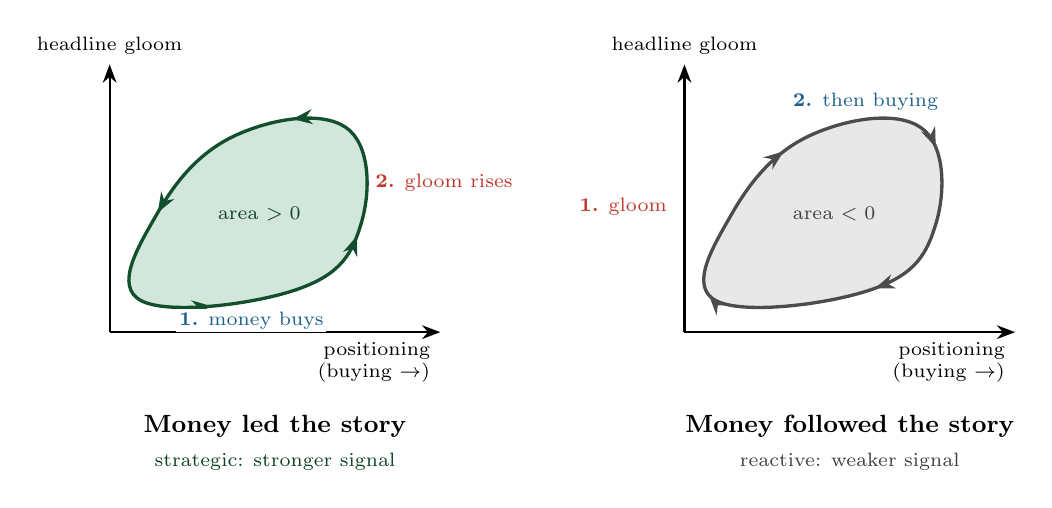
\begin{tikzpicture}[scale=1.0,
  arrowmid/.style={postaction={decorate}, decoration={markings,
    mark=at position 0.12 with {\arrow{Stealth[length=2.5mm]}},
    mark=at position 0.37 with {\arrow{Stealth[length=2.5mm]}},
    mark=at position 0.62 with {\arrow{Stealth[length=2.5mm]}},
    mark=at position 0.87 with {\arrow{Stealth[length=2.5mm]}}}}]
% left: money led
\begin{scope}
\draw[-{Stealth}, thick] (0,0) -- (4.2,0) node[below left, font=\scriptsize, align=right] {positioning\\(buying $\rightarrow$)};
\draw[-{Stealth}, thick] (0,0) -- (0,3.4) node[above, font=\scriptsize] {headline gloom};
\fill[good!20] plot[smooth cycle, tension=0.7] coordinates {(0.4,0.4) (2.4,0.55) (3.2,1.4) (3.0,2.6) (1.6,2.5) (0.6,1.5)};
\draw[good!60!black, very thick, arrowmid] plot[smooth cycle, tension=0.7] coordinates {(0.4,0.4) (2.4,0.55) (3.2,1.4) (3.0,2.6) (1.6,2.5) (0.6,1.5)};
\node[font=\scriptsize, text=good!50!black] at (1.9,1.5) {area $>0$};
\node[font=\scriptsize, anchor=north, text=do, fill=white, inner sep=1pt] at (1.8,0.3) {\textbf{1.} money buys};
\node[font=\scriptsize, anchor=west, text=echo] at (3.25,1.9) {\textbf{2.} gloom rises};
\node[font=\small\bfseries, align=center] at (2.1,-1.2) {Money led the story};
\node[font=\scriptsize, text=good!50!black] at (2.1,-1.65) {strategic: stronger signal};
\end{scope}
% right: money followed
\begin{scope}[xshift=7.3cm]
\draw[-{Stealth}, thick] (0,0) -- (4.2,0) node[below left, font=\scriptsize, align=right] {positioning\\(buying $\rightarrow$)};
\draw[-{Stealth}, thick] (0,0) -- (0,3.4) node[above, font=\scriptsize] {headline gloom};
\fill[gray!18] plot[smooth cycle, tension=0.7] coordinates {(0.4,0.4) (0.6,1.5) (1.6,2.5) (3.0,2.6) (3.2,1.4) (2.4,0.55)};
\draw[gray!60!black, very thick, arrowmid] plot[smooth cycle, tension=0.7] coordinates {(0.4,0.4) (0.6,1.5) (1.6,2.5) (3.0,2.6) (3.2,1.4) (2.4,0.55)};
\node[font=\scriptsize, text=gray!50!black] at (1.9,1.5) {area $<0$};
\node[font=\scriptsize, anchor=east, text=echo] at (-0.1,1.6) {\textbf{1.} gloom};
\node[font=\scriptsize, anchor=south, text=do] at (2.3,2.7) {\textbf{2.} then buying};
\node[font=\small\bfseries, align=center] at (2.1,-1.2) {Money followed the story};
\node[font=\scriptsize, text=gray!50!black] at (2.1,-1.65) {reactive: weaker signal};
\end{scope}
\end{tikzpicture}
\caption{Lead--lag as a loop. The direction of travel around the loop tells us who moved first; the enclosed area tells us how strongly.}
\label{fig:loop}
\end{figure}

% =====================================================================
\section{Putting It Together}

All signals feed a regime model that decides, event by event, which world we are in: \emph{informational} (money confirms the story: follow), \emph{overreaction} (mostly echo, no opposition: fade gently), or \emph{strategic} (money opposes the story and moved first: fade firmly). Each forecast comes with a calibrated confidence range \citep{gibbs2021}; a wide range means a small position.

\begin{figure}[ht]
\centering
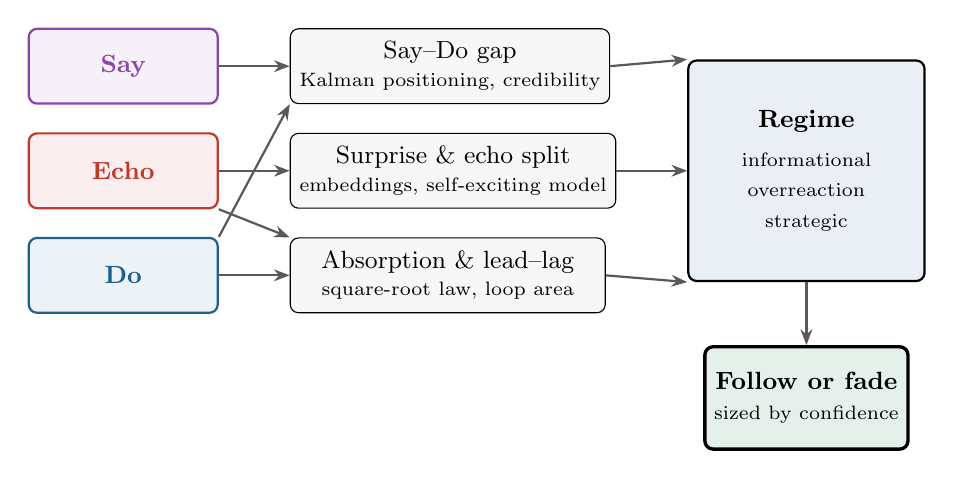
\begin{tikzpicture}[
  node distance=0.35cm and 0.9cm,
  voice/.style={draw, rounded corners=3pt, thick, minimum width=2.4cm, minimum height=0.95cm, align=center, font=\small\bfseries},
  sig/.style={draw, rounded corners=3pt, fill=gray!6, minimum width=4.0cm, minimum height=0.95cm, align=center, font=\small},
  arr/.style={-{Stealth[length=2mm]}, thick, gray!70!black}]
\node[voice, draw=say, fill=say!8, text=say] (say) {Say};
\node[voice, draw=echo, fill=echo!8, text=echo, below=of say] (echo) {Echo};
\node[voice, draw=do, fill=do!8, text=do, below=of echo] (do) {Do};
\node[sig, right=of say] (gap) {Say--Do gap\\[-1pt]\scriptsize Kalman positioning, credibility};
\node[sig, right=of echo] (news) {Surprise \& echo split\\[-1pt]\scriptsize embeddings, self-exciting model};
\node[sig, right=of do] (abs) {Absorption \& lead--lag\\[-1pt]\scriptsize square-root law, loop area};
\node[draw, rounded corners=3pt, thick, fill=do!10, minimum width=3.0cm, minimum height=2.8cm, align=center, font=\small, right=of news] (reg) {\textbf{Regime}\\[3pt]\scriptsize informational\\\scriptsize overreaction\\\scriptsize strategic};
\node[draw, rounded corners=3pt, very thick, fill=good!12, minimum width=2.4cm, minimum height=1.3cm, align=center, font=\small, below=0.8cm of reg] (dec) {\textbf{Follow or fade}\\\scriptsize sized by confidence};
\draw[arr] (say) -- (gap);
\draw[arr] (do.north east) -- (gap.south west);
\draw[arr] (echo) -- (news);
\draw[arr] (echo.south east) -- (abs.north west);
\draw[arr] (do) -- (abs);
\draw[arr] (gap.east) -- (reg.north west);
\draw[arr] (news) -- (reg);
\draw[arr] (abs.east) -- (reg.south west);
\draw[arr] (reg) -- (dec);
\end{tikzpicture}
\caption{The whole framework. Three voices become three families of signals, which a regime model turns into a single decision.}
\label{fig:pipeline}
\end{figure}

\begin{tcolorbox}[enhanced,breakable,colback=gray!4,colframe=gray!55!black,boxrule=0.6pt,arc=2pt,
  fonttitle=\bfseries\small,title={Illustration: a hypothetical downgrade},left=8pt,right=8pt]
\small
\textbf{Before.} Over eight days, call options build up, put skew flattens, and two directors buy shares.\\
\textbf{Day 0.} Two brokers downgrade the stock; coverage jumps from 15 stories a day to 140.

\begin{tabularx}{\linewidth}{@{}Xr@{}}
\toprule
Signal & Reading \\
\midrule
Sentiment surprise (new / echo) & $-0.5\sigma$ / $-2.3\sigma$: mostly echo \\
Say--Do gap & bearish words, bullish positioning \\
Expected vs actual reaction & $-6.0\%$ vs $-1.9\%$: strong absorption \\
Lead--lag loop & positive: money moved first \\
Regime (informational / overreaction / strategic) & 10\% / 28\% / 62\% \\
\bottomrule
\end{tabularx}

\textbf{Reading.} A probable false alarm. The framework leans long, but sizes modestly because the confidence range still includes losses.
\end{tcolorbox}

% =====================================================================
\section{What This Is, and What It Isn't}

\textbf{It measures disagreement, not intent.} A ``strategic'' reading means money and narrative moved in opposite directions in a particular order. It is not evidence that anyone lied, and large firms keep information barriers between research and trading.

\textbf{It is not blind contrarianism.} Real news is followed; only echo and contradicted narratives are faded.

\textbf{It uses only public information.} Creating or spreading narratives to move prices would itself be market manipulation. The framework reads the conversation; it never joins it.

\textbf{It is a concept, not yet a proven strategy.} Every component must be tested on point-in-time data before any capital is involved.

% =====================================================================
\begin{thebibliography}{99}\small
\bibitem[Bacry et al.(2015)]{bacry2015} Bacry, E., Mastromatteo, I., and Muzy, J.-F. (2015). Hawkes processes in finance. \emph{Market Microstructure and Liquidity}, 1(1).
\bibitem[Barber and Odean(2008)]{barber2008} Barber, B.~M., and Odean, T. (2008). All that glitters: The effect of attention and news on the buying behavior of individual and institutional investors. \emph{Review of Financial Studies}, 21(2), 785--818.
\bibitem[Bouchaud et al.(2018)]{bouchaud2018} Bouchaud, J.-P., Bonart, J., Donier, J., and Gould, M. (2018). \emph{Trades, Quotes and Prices}. Cambridge University Press.
\bibitem[Brunnermeier and Pedersen(2005)]{brunnermeier2005} Brunnermeier, M.~K., and Pedersen, L.~H. (2005). Predatory trading. \emph{Journal of Finance}, 60(4), 1825--1863.
\bibitem[Chan(2003)]{chan2003} Chan, W.~S. (2003). Stock price reaction to news and no-news: Drift and reversal after headlines. \emph{Journal of Financial Economics}, 70(2), 223--260.
\bibitem[Chevyrev and Kormilitzin(2016)]{chevyrev2016} Chevyrev, I., and Kormilitzin, A. (2016). A primer on the signature method in machine learning. arXiv:1603.03788.
\bibitem[De Long et al.(1990)]{delong1990} De Long, J.~B., Shleifer, A., Summers, L.~H., and Waldmann, R.~J. (1990). Noise trader risk in financial markets. \emph{Journal of Political Economy}, 98(4), 703--738.
\bibitem[Gibbs and Cand\`es(2021)]{gibbs2021} Gibbs, I., and Cand\`es, E. (2021). Adaptive conformal inference under distribution shift. \emph{NeurIPS}, 34.
\bibitem[Hawkes(1971)]{hawkes1971} Hawkes, A.~G. (1971). Spectra of some self-exciting and mutually exciting point processes. \emph{Biometrika}, 58(1), 83--90.
\bibitem[van den Oord et al.(2018)]{oord2018} van den Oord, A., Li, Y., and Vinyals, O. (2018). Representation learning with contrastive predictive coding. arXiv:1807.03748.
\bibitem[Shleifer and Vishny(1997)]{shleifer1997} Shleifer, A., and Vishny, R.~W. (1997). The limits of arbitrage. \emph{Journal of Finance}, 52(1), 35--55.
\bibitem[Tetlock(2007)]{tetlock2007} Tetlock, P.~C. (2007). Giving content to investor sentiment: The role of media in the stock market. \emph{Journal of Finance}, 62(3), 1139--1168.
\end{thebibliography}

\end{document}
